\section{Travail en groupe}
Ce projet nous a permis de goûter à la réalisation d'un travail sur un sujet poussé et nouveau, et ce sur une longue durée et en groupe. Cela nous a donc poussé à parfaire notre adaptation, que ce soit au niveau de notre emploi du temps, ou même par rapport aux autres membres du groupe. Les prises de décisions, l'organisation, et les méthodes pour mettre à bien notre projet étaient à décider en équipe, ce qui nous a aussi permi de nouer des liens entre nous. La grande majorité du groupe étant jeune, et fraîchement sortie du lycée, les concepts de managment d'équipe et d'abnégation pour réaliser un travail étaient nouveaux, et très enrichissants pour des étudiants comme nous.

Aussi, nous avons evidemment dû surmonter de multiples difficultés, au fil de la réalisation du robot.

La soudure étant une pratique totalement nouvelle pour tous, nous avons dû prendre un certain temps afin de la maîtriser du moins assez correctement pour la pratiquer directement sur nos propres cartes. Elle a donc été source de plusieurs soucis au long du projet. Certains points de soudures ont parfois été mal réalisés, des composants placés à l'envers ont créé des court circuits que nous avons  dû nous même identifier, etc.

Le suivi de projet, a été tenu sur GitHub, afin de pouvoir centraliser les documents du groupe.

\begin{figure}[H]
\centering
\begin{minipage}{.5\textwidth}
  \centering
\href{}{}  \centerline{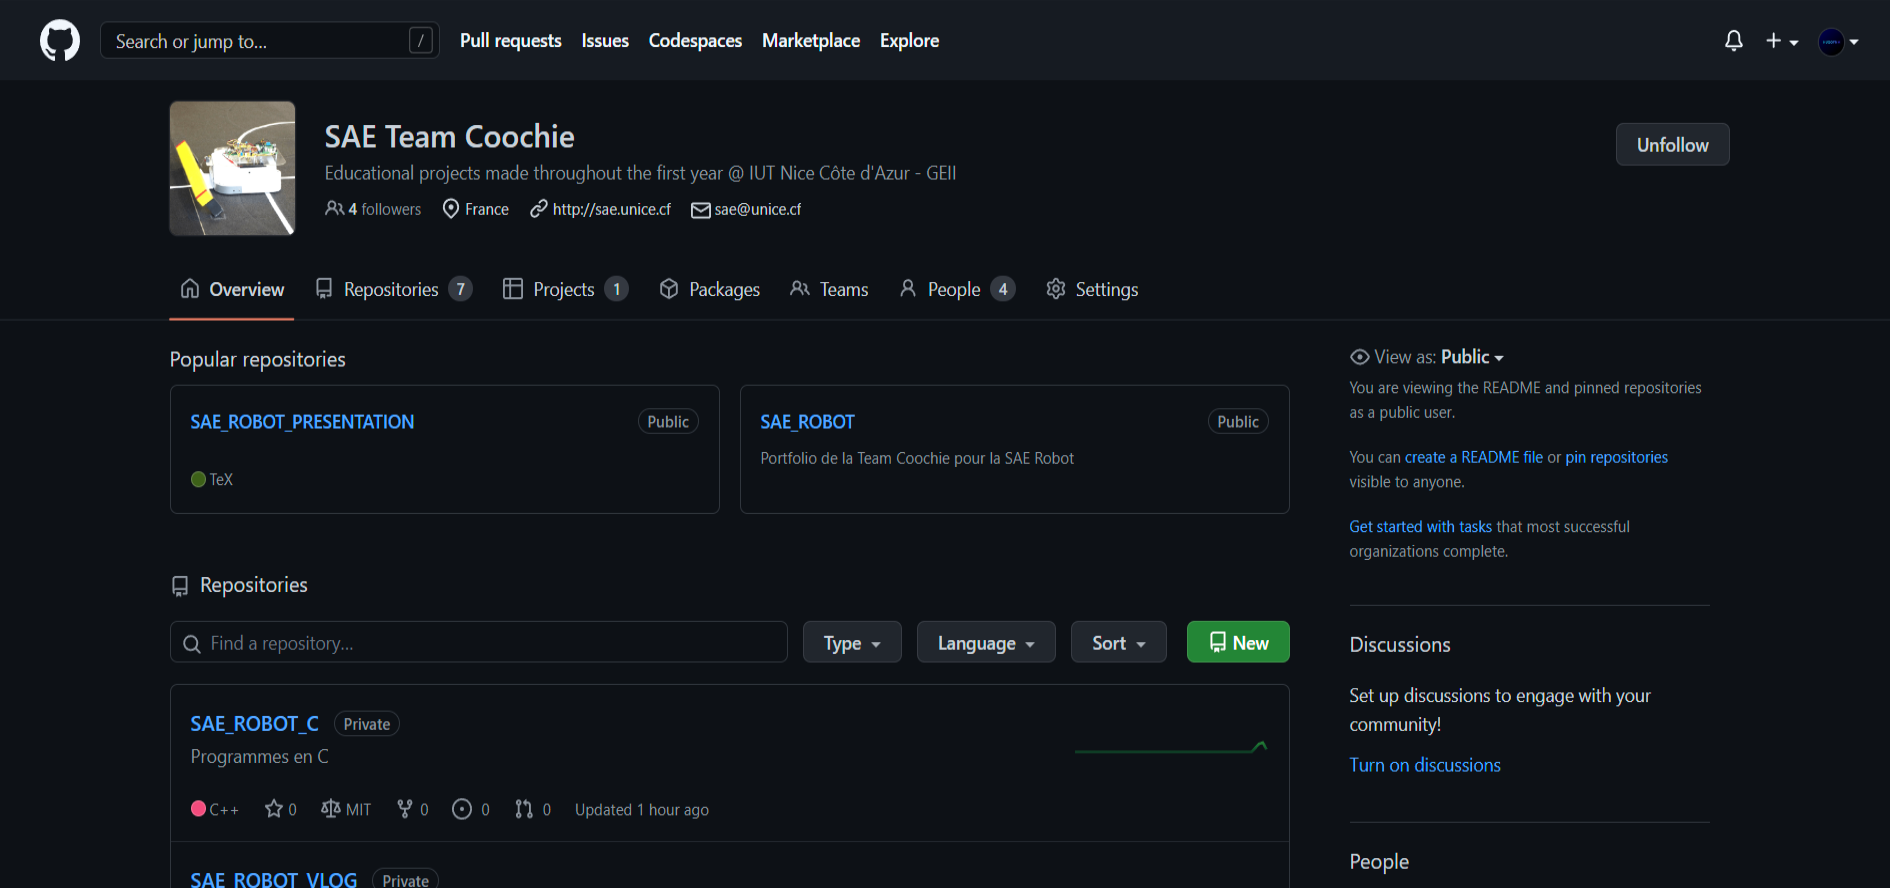
\includegraphics[width=2\linewidth]{img/sex.png}}
  \captionof{figure}{\emph{Logiciel de gestion de versions GitHub basé sur git.}}
  \label{fig:git}
\end{minipage}%
\end{figure}

\vfill
\noindent\makebox[\linewidth]{\rule{.8\paperwidth}{.6pt}}\\[0.2cm]
I.U.T. Nice Côte d'Azur - SAE Robot - 2023 \hfill goofyBot
\noindent\makebox[\linewidth]{\rule{.8\paperwidth}{.6pt}}
\newpage

\begin{figure}[H]
\centering
\begin{minipage}{.5\textwidth}
  \centering
\href{}{}  \centerline{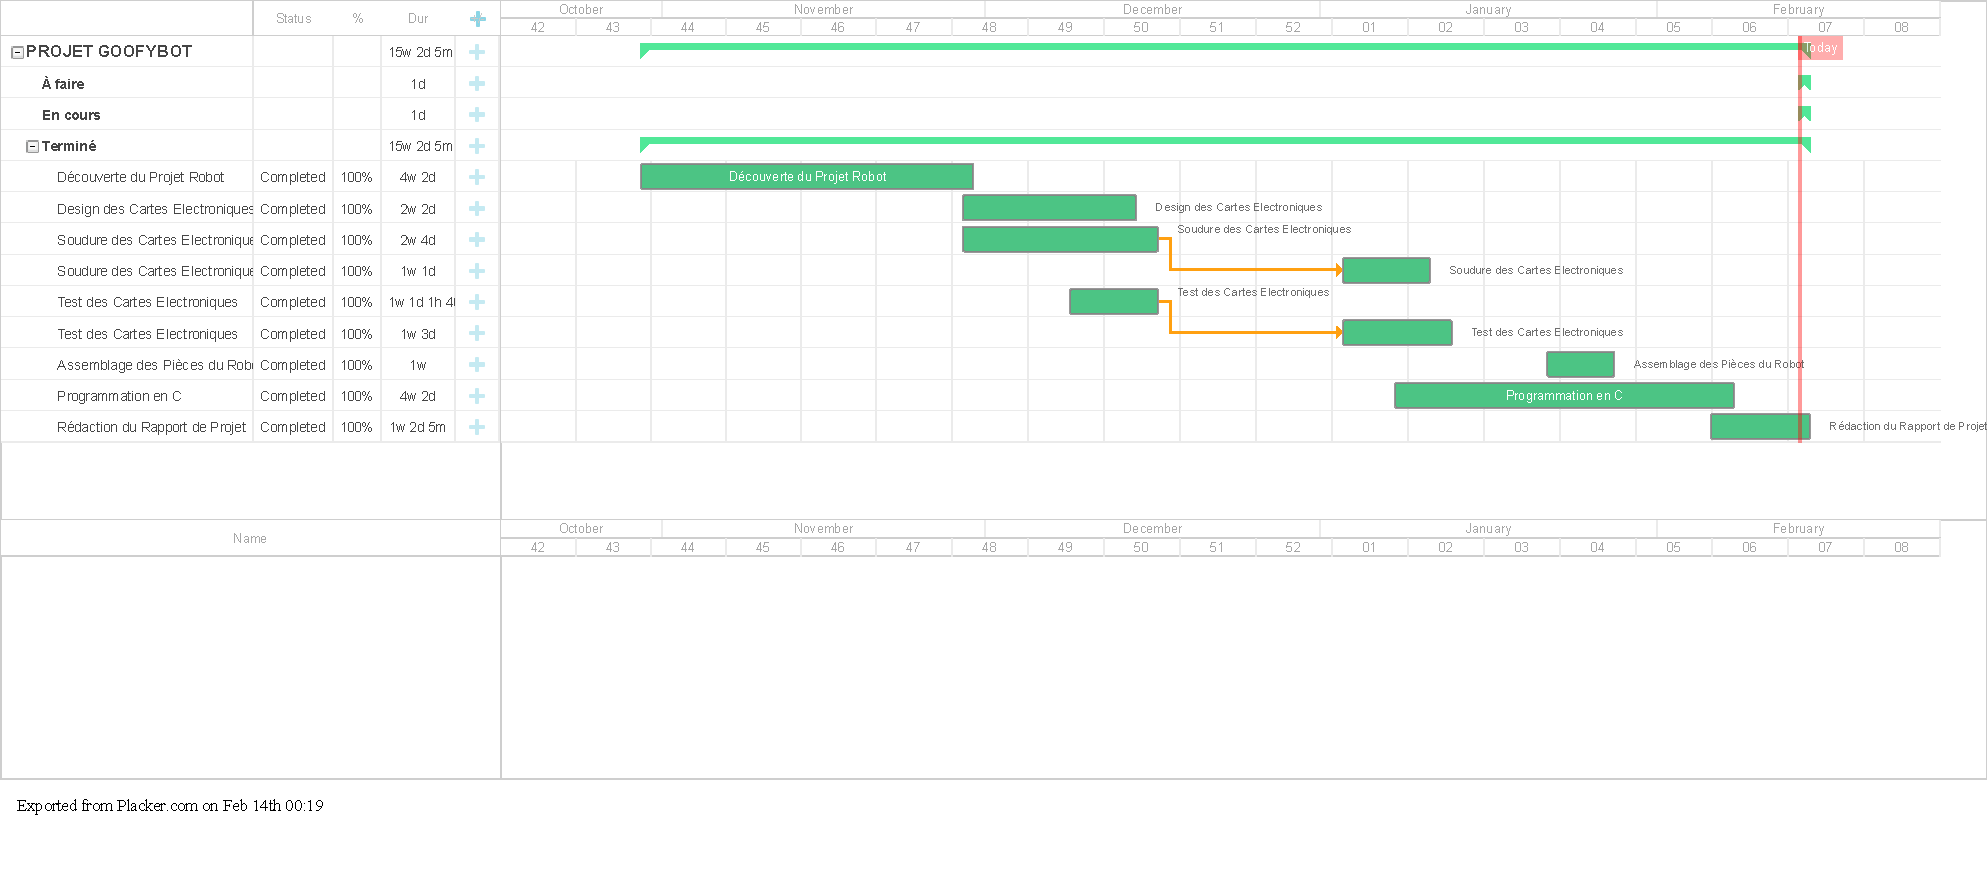
\includegraphics[width=2.5\linewidth]{pdf/gantt.pdf}}
  \captionof{figure}{\emph{GANTT.}}
  \label{fig:gantt}
\end{minipage}%
\end{figure}


\begin{figure}[H]
\centering
\begin{minipage}{.5\textwidth}
  \centering
  \centerline{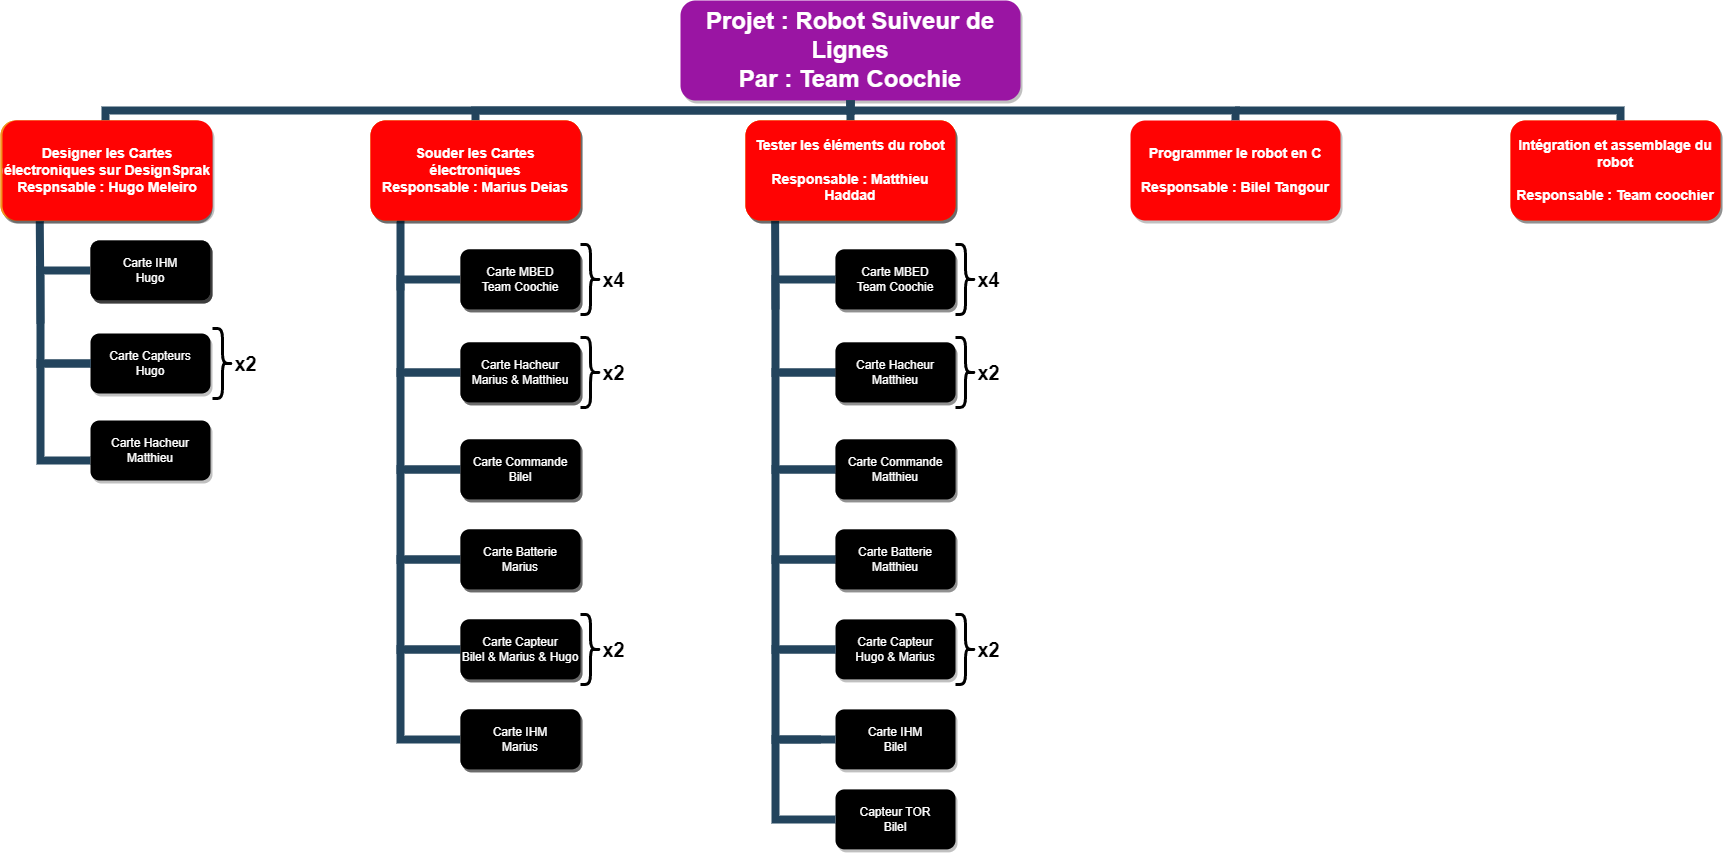
\includegraphics[width=2.5\linewidth]{img/obs.png}}
  \captionof{figure}{\emph{OBS.}}
  \label{fig:obs}
\end{minipage}%
\end{figure}

\vfill
\noindent\makebox[\linewidth]{\rule{.8\paperwidth}{.6pt}}\\[0.2cm]
I.U.T. Nice Côte d'Azur - SAE Robot - 2023 \hfill goofyBot
\noindent\makebox[\linewidth]{\rule{.8\paperwidth}{.6pt}}
\newpage